\section{IMU}
The previous odometry measuring device, the MPU6250 \cite{mpu6250} was broken, which is why a new, updated version is currently being used.
Another reason a new version is used is that the MPU9250 \cite{MPU9250} also contains an AK8963, which is a 3-axis magnetometer.
This allow WTR to more accurately track orientation, since it can use the magnetometer to find its position relative to the north.
The data is collected as explained in this section \ref{sec::collect}, and then transmitted to a Raspberry Pi which deals with all the sensors.
After that has processed the data into a ROS standard message, it sends the data on to the topic, where it can then be used by planners.

\subsection{Collecting data} \label{sec::collect}
The main controller for collecting the data is an Arduino Uno, which uses I$^{2}$C for communication with the MPU9250.
The clock is set at 400000, and the address uses the \code{MPU9250\_ADDRESS\_AD0}, a macro which determines the supposed address.
In section \ref{sec::set-up}, the curiosities of the address are further explained.
The Arduino takes the raw data, and uses \href{https://github.com/sparkfun/SparkFun_MPU-9250_Breakout_Arduino_Library}{this library} to process the data.
This is needed because the MPU does not output quaternions by default.
This library allows the Arduino to calculate those, and then send them on to the Pi.


\subsubsection{The Set-up} \label{sec::setup}
After checking the address of the MPU9250, it will first do a self-test, where it determines the biases and stores them in its registers, through the \code{MPU9250SelfTest()} and \code{calibrateMPU9250()} functions.
The address of the MPU should be 0x71 according to the library, but since a slightly different model is used from the one the demo code is written for, the address is 0x73.
After that, it calibrates itself and stores those values as well.
Following that, it is fully initialized using the \code{initMPU9250} function.

After that, it checks what the address of the AK8693 (the magnetometer), and if that is not 0x48, it cancels the entire system.
Thankfully, this address does match the default in the library provided.
The AK8963 is initialized, and the resolutions of the 3 different sensors are fetched using \code{getAres(), getGres(), and getMres()}.
This concludes the set-up.


\subsubsection{The Loop}
The core concept of the loop is relatively simple, were it not for some of the quaternion calculations.
First it reads the data gathered by the IMU, and stores it in 3 arrays, one per sensor.
This data is then transformed, though differently per sensor.
The accelerometer data is changed to acceleration in $m/s^2$, and the gyroscopic data is calculated into degrees per second.
The magnetometer data does not get changed much, except for the compensation for the biases.

This data is then calculated into a quaternion, using the Madgwick calculation.
This is very complicated, and better to be considered as a black box.
Should you wish to learn about them anyway, consider checking out \href{http://www.ijcee.org/vol10/974-T4004.pdf}{this link}.
This does require an understanding of imaginary numbers, complex numbers, and matrix calculations.
A good source of information on those can be found \href{https://www.3dgep.com/understanding-quaternions/#The_Complex_Plane}{here.}

Of course, all the collected data in the world does not do any good if it is not transmitted, and the details on that are explained in the next section.

\subsection{Arduino to Pi protocol}
The order in which the data is sent is naturally important.
The raspberry Pi expects the data packet to start with "\$ 0x03", and then the data of the quaternion, the gyroscope, the accelerometer, the temperature and lastly the magnetometer. 

Most of the program used to interface with the MPU9250 is based on a program by sparkfun, \cite{sparkfunMPU9250}, which is in turn based on the code by KrisWiner on Github \cite{kriswiner}.
Several parts have been stripped out, since no LCD is used.
Additionally, any debug messages have been removed after confirming that the code runs consistently.

Each of the sensors returns a 16 bit piece of data, as a signed 16-bit integer.
The exception to this rule is the quaternion calculation.
For that, a float with the values ranging between -1 and +1 can be expected.
Quaternions are rather tricky to work with, but more explanation can be found \href{https://www.3dgep.com/understanding-quaternions/#The_Complex_Plane}{here.}
As a quick warning, this is rather complex math, using both imaginary numbers and matrices.
It is worthwhile to study, since they form an integral part of the message to ROS.

As serial communications are used, the data cannot be transmitted as is.
In order to combat this, the data is split into two parts, with the quaternion again being an exception.
The two 8-bit unsigned integers are then transmitted, with the 8 bits representing the MSB \ref{trm::MSB} first and the LSB \ref{trm::LSB} last.
These two integers are then spliced back into a signed 16-bit integer once the Pi has received them.


\begin{figure}[H]
    \begin{lstlisting}[language=c++,firstnumber=0]
        [ start byte ] = '$'
        [ start byte ] = 0x03
        [ quaternion value W ] = quaternion value from -1 to +1, multiplied by 100
        [ quaternion value X ]
        [ quaternion value Y ]
        [ quaternion value Z ]
        [ accelerometer X byte 1 ]
        [ accelerometer X byte 2 ]
        [ accelerometer X byte 3 ]
        [ accelerometer X byte 4 ]
        [ accelerometer Y byte 1 ]
        [ accelerometer Y byte 2 ]
        [ accelerometer Y byte 3 ]
        [ accelerometer Y byte 4 ]
        [ accelerometer Z byte 1 ]
        [ accelerometer Z byte 2 ]
        [ accelerometer Z byte 3 ]
        [ accelerometer Z byte 4 ]
        [ gyroscope X byte 1 ] 
        [ gyroscope X byte 2 ]
        [ gyroscope X byte 3 ]
        [ gyroscope X byte 4 ]       
        [ gyroscope Y byte 1 ] 
        [ gyroscope Y byte 2 ]
        [ gyroscope Y byte 3 ]
        [ gyroscope Y byte 4 ] 
        [ gyroscope Z byte 1 ] 
        [ gyroscope Z byte 2 ]
        [ gyroscope Z byte 3 ]
        [ gyroscope Z byte 4 ] 
        [ magnetometer X byte 1 ]
        [ magnetometer X byte 2 ]
        [ magnetometer X byte 3 ]
        [ magnetometer X byte 4 ]
        [ magnetometer Y byte 1 ]
        [ magnetometer Y byte 2 ]
        [ magnetometer Y byte 3 ]
        [ magnetometer Y byte 4 ]
        [ magnetometer Z byte 1 ]
        [ magnetometer Z byte 2 ]
        [ magnetometer Z byte 3 ]
        [ magnetometer Z byte 4 ]
        [ message count ]
        [ '\r' ] 
        [ '\n' ] 
    \end{lstlisting} 
\caption{The order the Pi expects the data it receives to have}
\label{fig::dataformat}
\end{figure}

\subsection{Reception on the Pi}
Naturally, the data has to be sent somewhere.
In this case, the sensor Pi is responsible for handling this data.
After receiving all the data, it sends the messages to the appropriate ROS topics.

First, it creates node handles and message objects that will be used to transmit the relevant data.
The ROS communication rate is set at 200Hz, which is more than sufficient.
The covariances are set, though for the magnetometer they are as of yet unknown.
ROS uses 0.01 as a default value, since the covariance is not noted in any data-sheets, and the calculations to find them are almost a study onto themselves.

The basic process is shown in figure \ref{fig::piDataReception}.

\begin{figure}[H]
\centering
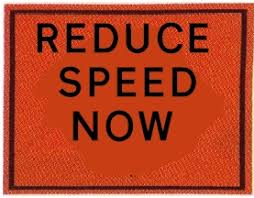
\includegraphics[width=12cm]{temp.jpg}
\caption{The process by which incoming data is handled on the Pi}
\label{fig::piDataReception}
\end{figure}

The data recorded by the arduino is stored in a float data-type, which is not transmittable by serial communications.
In order to counter this, all the floats are split into 4 bytes, each stored in an array of 4 unsigned 8-bit integers.
This is then read byte for byte, and each time the already existing result is left shifted by 8, so that after 4 iterations the full float is back again.
These floats are still raw data, however.
In order to ensure they are ROS compliant \cite{ROSformat}, they are changed into the appropriate units, such as radians and $ms^{-2}$, rather than the degrees and G's they are returned as by the MPU9250 \cite{MPU9250}.

This is done, for the accelerometer data, by multiplying it by the standard for gravity on earth, 9.81.
This converts it from G's into $ms^{-2}$.
For the gyroscope, the data needs to be in radians, which is achieved by multiplying the degrees by $\pi$, and then dividing it by 180.
The magnetometer data is a bit simpler, since the difference between milliGauss and Tesla is just a matter of factor.
One Tesla is $1.0 \cdot 10^{7}$ milliGauss, so in order to convert mG into T, the opposite needs to be done, multiplying the received data by  $1.0 \cdot 10^{-7}$.

The message number is used to keep track of whether or not any packages are missed, if there are missed packages a warning is shown in the ROS debug screen.
If the message number is the same, then another warning is shown because it is likely the arduino running the MPU9250 has crashed.


\newpage